%LaTeX template : http://systbio.org/files/SB_LaTeX_Template_txt_extension.txt
%Author instructions: http://www.oxfordjournals.org/our_journals/sysbio/for_authors/ms_preparation.html

\documentclass[12pt,letterpaper]{article}
\usepackage{natbib}

%Packages
\usepackage{pdflscape}
\usepackage{fixltx2e}
\usepackage{textcomp}
\usepackage{fullpage}
\usepackage{float}
\usepackage{latexsym}
\usepackage{url}
\usepackage{epsfig}
\usepackage{graphicx}
\usepackage{amssymb}
\usepackage{amsmath}
\usepackage{bm}
\usepackage{array}
\usepackage[version=3]{mhchem}
\usepackage{ifthen}
\usepackage{caption}
\usepackage{hyperref}
\usepackage{amsthm}
\usepackage{amstext}
\usepackage{enumerate}
\usepackage[osf]{mathpazo}
\usepackage{dcolumn}
\usepackage{lineno}
\usepackage{dcolumn}
\newcolumntype{d}[1]{D{.}{.}{#1}}

\pagenumbering{arabic}


%Pagination style and stuff
\linespread{2}
\raggedright
\setlength{\parindent}{0.5in}
\setcounter{secnumdepth}{0} 
\renewcommand{\section}[1]{%
\bigskip
\begin{center}
\begin{Large}
\normalfont\scshape #1
\medskip
\end{Large}
\end{center}}
\renewcommand{\subsection}[1]{%
\bigskip
\begin{center}
\begin{large}
\normalfont\itshape #1
\end{large}
\end{center}}
\renewcommand{\subsubsection}[1]{%
\vspace{2ex}
\noindent
\textit{#1.}---}
\renewcommand{\tableofcontents}{}

\begin{document}

%Running head
\begin{flushright}
Version dated: \today
\end{flushright}
\bigskip
\bigskip
\medskip
\begin{center}

\noindent{\Large \bf Mammalian morphological diversity does not increase in response to the Cretaceous-Paleogene (K-Pg) extinction event and the extinction of the (non-avian) dinosaurs.} 
% NC: still think this might need some work

\bigskip

\noindent {\normalsize \sc Thomas Guillerme$^1$$^,$$^2$$^*$, and Natalie Cooper$^1$$^,$$^2$$^,$$^3$}\\
\noindent {\small \it 
$^1$School of Natural Sciences, Trinity College Dublin, Dublin 2, Ireland.\\
$^2$Trinity Centre for Biodiversity Research, Trinity College Dublin, Dublin 2, Ireland.\\
$^3$Department of Life Sciences, Natural History Museum, Cromwell Road, London, SW7 5BD, UK.}\\
\end{center}
\medskip
\noindent{*\bf Corresponding author.} \textit{Zoology Building, Trinity College Dublin, Dublin 2, Ireland; E-mail: guillert@tcd.ie; Fax: +353 1 6778094; Tel: +353 1 896 2571.}\\
\vspace{1in}

%Line numbering
\modulolinenumbers[1]
\linenumbers

\renewcommand\thefigure{S\arabic{figure}}
\renewcommand\thetable{S\arabic{table}}

\section{Supplementary results}

\subsection{Phylogenies}
This section contains the trimmed phylogenies used in the analysis (see methods section in the main text for details).
% TG: this strap package is pure coded sweetness... I love these phylogenies!
\begin{figure}[!htbp]
\centering
    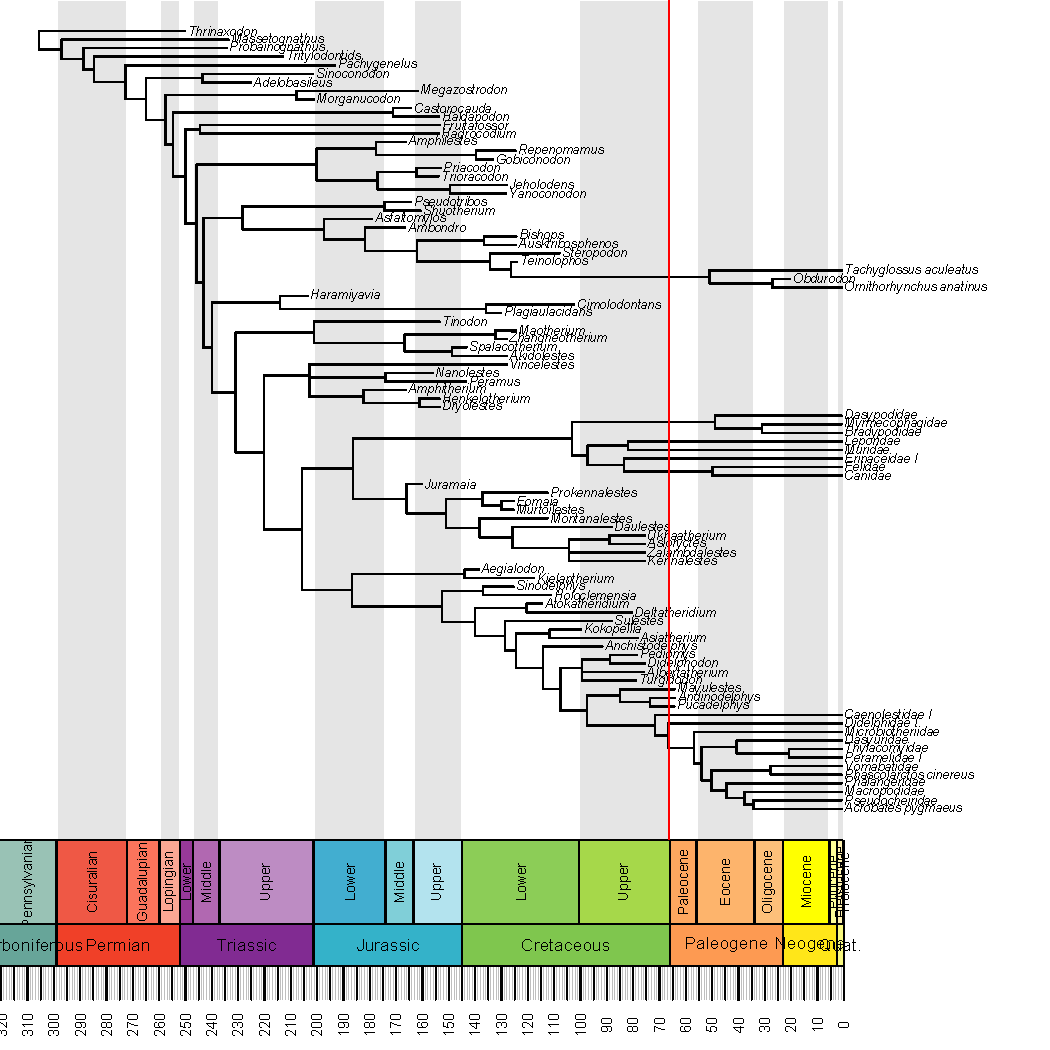
\includegraphics[keepaspectratio=true]{Figures/Slater_tree.pdf}
\caption{Mammaliaformes phylogeny from \cite{Slater2012MEE}. The phylogeny only contains taxa with overlapping cladistic data. The vertical red line represents the K-Pg boundary.}
\end{figure}

\begin{figure}[!htbp]
\centering
    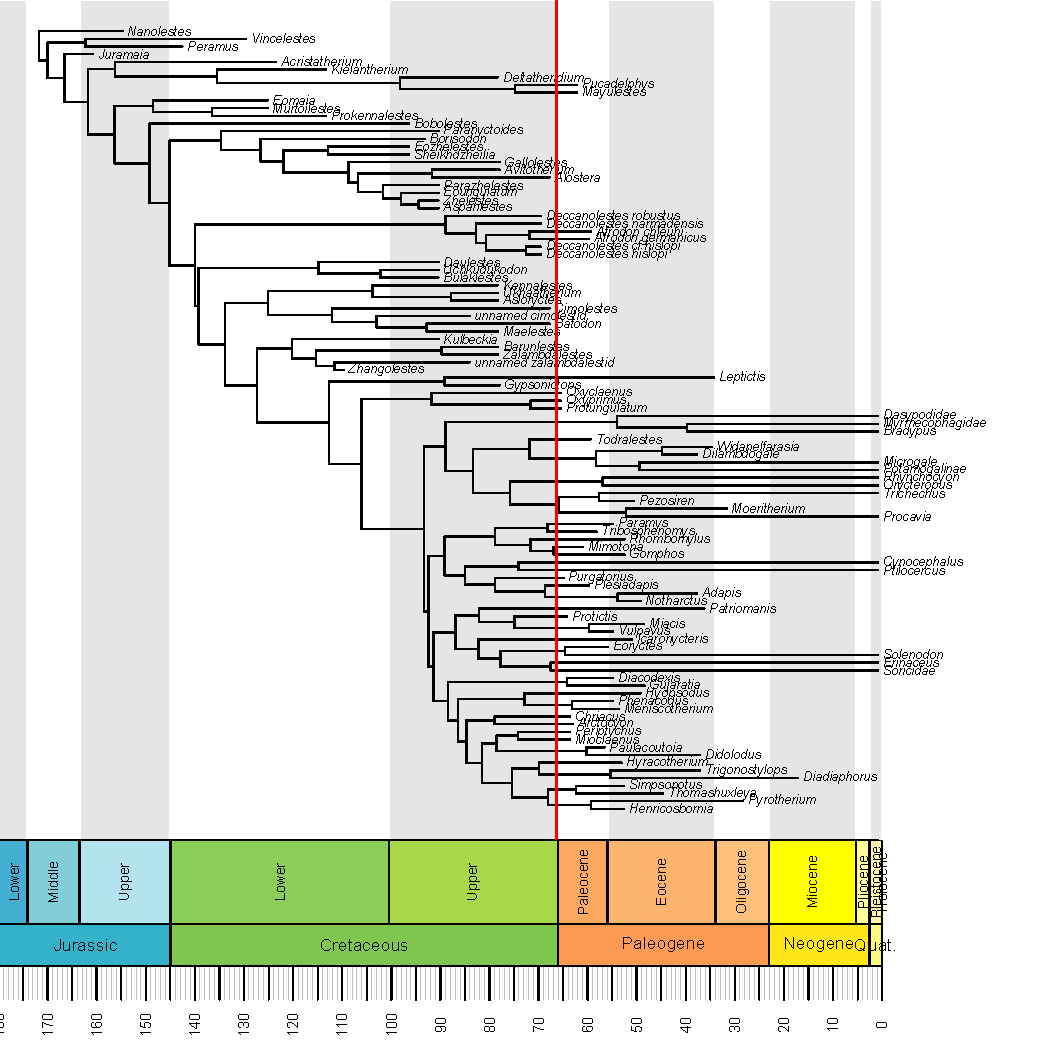
\includegraphics[keepaspectratio=true]{Figures/Beck_tree.pdf}
\caption{Eutherian phylogeny from \cite{beckancient2014}. The phylogeny only contains taxa with overlapping cladistic data. The vertical red line represents the K-Pg boundary.}
\end{figure}

\subsection{Rarefied analysis}
This section contains the results from the rarefied Mammaliaformes and Eutheria datasets (see methods section in the main text for details).

\begin{figure}[!htbp]
\centering
    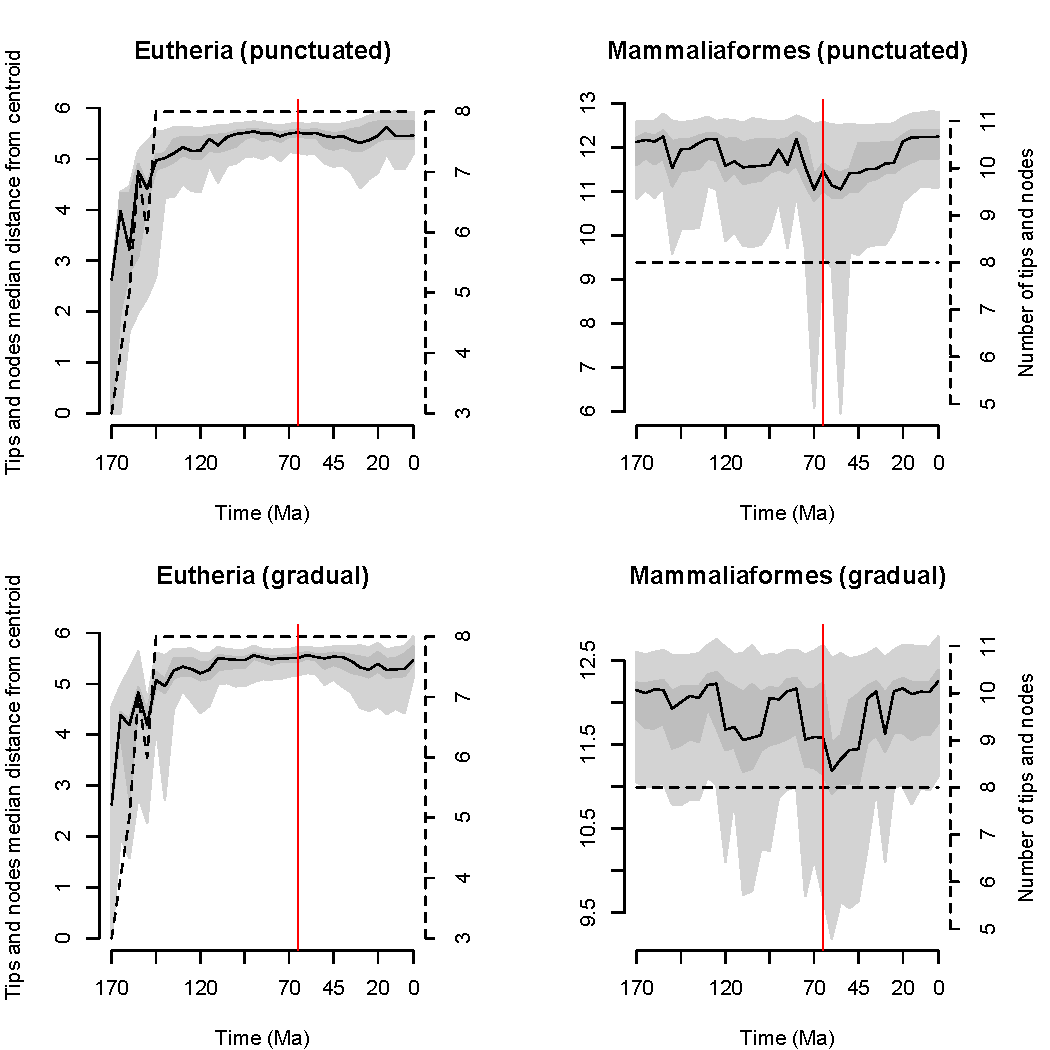
\includegraphics[keepaspectratio=true]{Figures/Main_results_rarefied.pdf}
\caption{Disparity through time in Eutheria and Mammaliaformes calculated using a model of punctuated or gradual evolution, but controlling for variations in species richness at each time slice using rarefaction. The x axis represents time in millions of years before the present (Ma). The y axis represents disparity, measured as the median distance from centroid at each time slice.
 The solid black lines show the mean disparity estimated from 1000 bootstrapped pseudoreplicates; the confidence intervals (CI) are represented by the grey polygons (50\% CI in dark grey and 95\% CI in light grey). The right hand axis represents species richness, and the dashed line shows the species richness in each time slice. The red vertical line indicates the Cretaceous-Paleogene (K-Pg) boundary (66 Ma).}
\label{fig:Fig_Rar_results}
\end{figure}


\begin{table}[ht]
\caption{Results of comparing the rarefied disparity at the last subsample of the Cretaceous (70 Ma) to the subsamples of the Paleocene and Eocene the Eutheria dataset under both gradual and punctuated evolutionary models. Difference: mean subsample difference; df: degrees of freedom; t: t statistic.}
\label{tab:Tab_beck}
\centering
\begin{tabular}{r|cccc|cccc}
  \hline
  Compared & \multicolumn{4}{c|}{Gradual model} & \multicolumn{4}{c}{Punctuated model} \\
  subsamples & difference & df & t & p value & difference & df & t & p value \\ 
  \hline
  70 \textit{vs.} 65 Ma & -0.030 & 84 & -0.169 & 0.866 & 0.030 & 84 & 0.167 & 0.868 \\ 
  70 \textit{vs.} 60 Ma & 0.010 & 76 & 0.030 & 0.976 & 0.040 & 76 & 0.260 & 0.795 \\ 
  70 \textit{vs.} 55 Ma & 0.010 & 75 & 0.039 & 0.969 & 0.010 & 75 & 0.031 & 0.976 \\ 
  70 \textit{vs.} 50 Ma & 0.080 & 68 & 0.409 & 0.684 & 0.130 & 68 & 0.686 & 0.495 \\ 
  70 \textit{vs.} 45 Ma & 0.120 & 64 & 0.550 & 0.584 & 0.100 & 64 & 0.550 & 0.584 \\ 
  70 \textit{vs.} 40 Ma & 0.100 & 64 & 0.465 & 0.644 & 0.140 & 64 & 0.695 & 0.490 \\ 
  70 \textit{vs.} 35 Ma & 0.110 & 60 & 0.476 & 0.636 & 0.090 & 60 & 0.464 & 0.644 \\ 
   \hline
\end{tabular}
\end{table}

\begin{table}[ht]
\caption{Results of comparing the rarefied disparity at the last subsample of the Cretaceous (70 Ma) to the subsamples of the Paleocene and Eocene the Mammaliaformes dataset under both gradual and punctuated evolutionary models. Column heads explained same as given in Table ~\ref{tab:Tab_beck}.}
\label{tab:Tab_slater}
\centering
\begin{tabular}{r|cccc|cccc}
  \hline
  Compared & \multicolumn{4}{c|}{Gradual model} & \multicolumn{4}{c}{Punctuated model} \\
  subsamples & Difference & Df & T & p value & Difference & Df & T & p value \\ 
  \hline
  70 \textit{vs.} 65 Ma & -0.440 & 21 & -0.561 & 0.581 & -0.240 & 21 & -0.405 & 0.690 \\ 
  70 \textit{vs.} 60 Ma & -0.150 & 18 & -0.162 & 0.873 & 0.220 & 18 & 0.305 & 0.764 \\ 
  70 \textit{vs.} 55 Ma & -0.120 & 19 & -0.130 & 0.898 & 0.150 & 19 & 0.213 & 0.834 \\ 
  70 \textit{vs.} 50 Ma & -0.330 & 20 & -0.405 & 0.690 & -0.170 & 20 & -0.277 & 0.785 \\ 
  70 \textit{vs.} 45 Ma & -0.390 & 23 & -0.509 & 0.616 & -0.220 & 23 & -0.342 & 0.736 \\ 
  70 \textit{vs.} 40 Ma & -0.500 & 24 & -0.668 & 0.510 & -0.310 & 24 & -0.570 & 0.574 \\ 
  70 \textit{vs.} 35 Ma & -0.560 & 26 & -0.740 & 0.466 & -0.230 & 26 & -0.360 & 0.722 \\ 
   \hline
\end{tabular}
\end{table}

\begin{figure}[!htbp]
\centering
    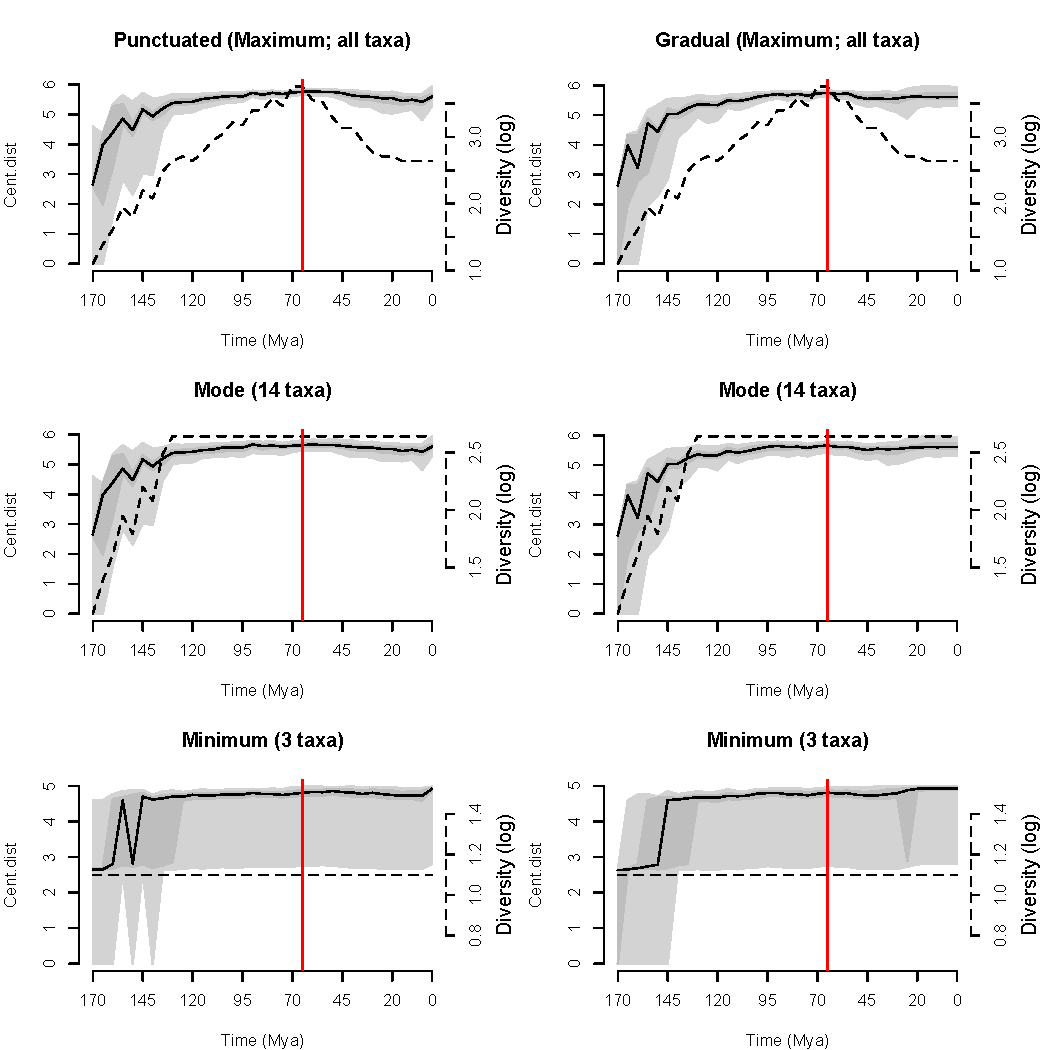
\includegraphics[keepaspectratio=true]{Figures/Rarefaction(beck).pdf}
\caption{Variations of disparity through time among Eutherian with a punctuated or gradual evolution model for different number of taxa (rarefaction). The x axis represents the time in Million of years ago (Mya). The y axis represents the disparity measured as the median distance from centroid per sub-sample. The solid black lines is the mean disparity; the confidence intervals (CI) are represent by the grey polygons (50\% CI in dark grey and 95\% CI in light grey). The dashed line represent the species richness in each sub-sample (values are reported on the right hand side of each graphs). The red vertical line represents the K-Pg boundary (66 Mya).}
\end{figure}

\begin{figure}[!htbp]
\centering
    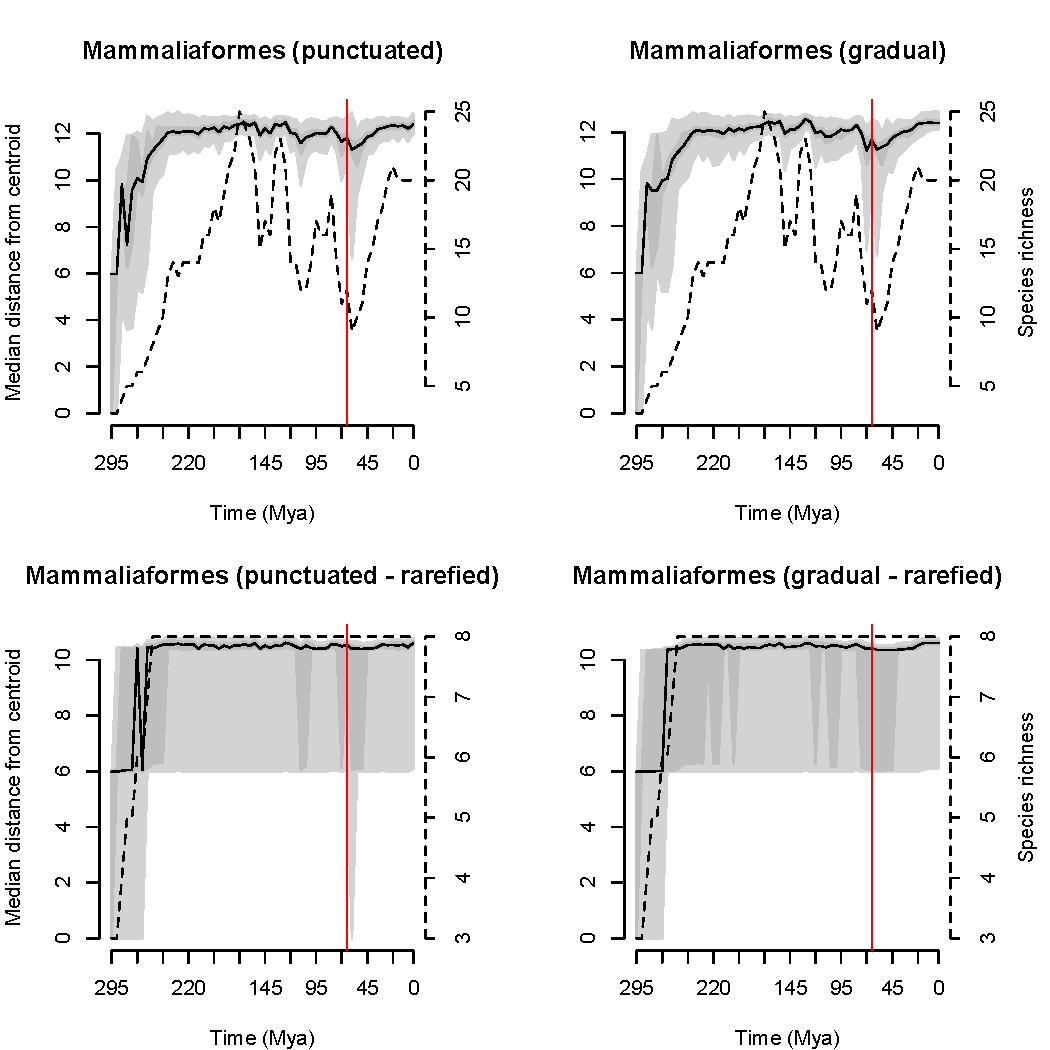
\includegraphics[keepaspectratio=true]{Figures/Slater_full.pdf}
\caption{Observed and rarefied variation of disparity through time among Mammaliaformes with a punctuated or gradual evolution model. The x axis represents the time in Million of years ago (Mya). The y axis represents the disparity measured as the median distance from centroid per sub-sample. The solid black lines is the mean disparity; the confidence intervals (CI) are represent by the grey polygons (50\% CI in dark grey and 95\% CI in light grey). The dashed line represent the species richness in each sub-sample (values are reported on the right hand side of each graphs). The red vertical line represents the K-Pg boundary (66 Mya).}
\end{figure}


\subsection{Other disparity measurements}
This section contains the results of the analysis of the Mammaliaformes and Eutherian data set with all the disparity measurements and methods for sampling disparity through time.
The different disparity measurements are the median distance from centroid (see methods section in the main text for details) as well as the median sum and products of ranges and variances from \cite{Wills1994}.
The different methods for sampling disparity through time are:
\begin{enumerate}
\item \textbf{Intervals (tips only)}. We selected every tips present at every stages from the early Middle Jurassic (Bajocian, starting at 170.3 Mya) to the present. We collapsed together every stage containing less than 3 tips. Note that some tips where present in multiple stages due to their occurrence data (see methods section in the main text for details on the occurrence data).
\item \textbf{Intervals (tips and nodes)}. We selected every stage tips and nodes present at every stages from the early Middle Jurassic (Bajocian, starting at 170.3 Mya) to the present. We collapsed together every stage containing less than 3 elements (tips and/or nodes).
\item \textbf{Slices (punctuated)}. These are the results presented in the main text where time is sample equidistantly and evolution is assumed to be punctuated (randomly selecting either data from the descendant or the ancestor when slicing through a branch; see methods section in the main text for details).
\item \textbf{Slices (punctuated: acctran)}. Similar as slices (punctuated) method but data is always selected from the descendant (see methods section in the main text for details).
\item \textbf{Slices (punctuated: deltran)}. Similar as slices (punctuated) method but data is always selected from the ancestor (see methods section in the main text for details).
\item \textbf{Slices (gradual)}. SThese are the results presented in the main text where time is sample equidistantly and evolution is assumed to be gradual (data is selected from the descendant or the ancestor based on branch length; see methods section in the main text for details).
\end{enumerate}
We also rarefied both data sets for all the metrics and all the methods using only 3 taxa for the interval methods and 8 taxa for the slices methods.


\begin{landscape}
\begin{figure}[!htbp]
\centering
    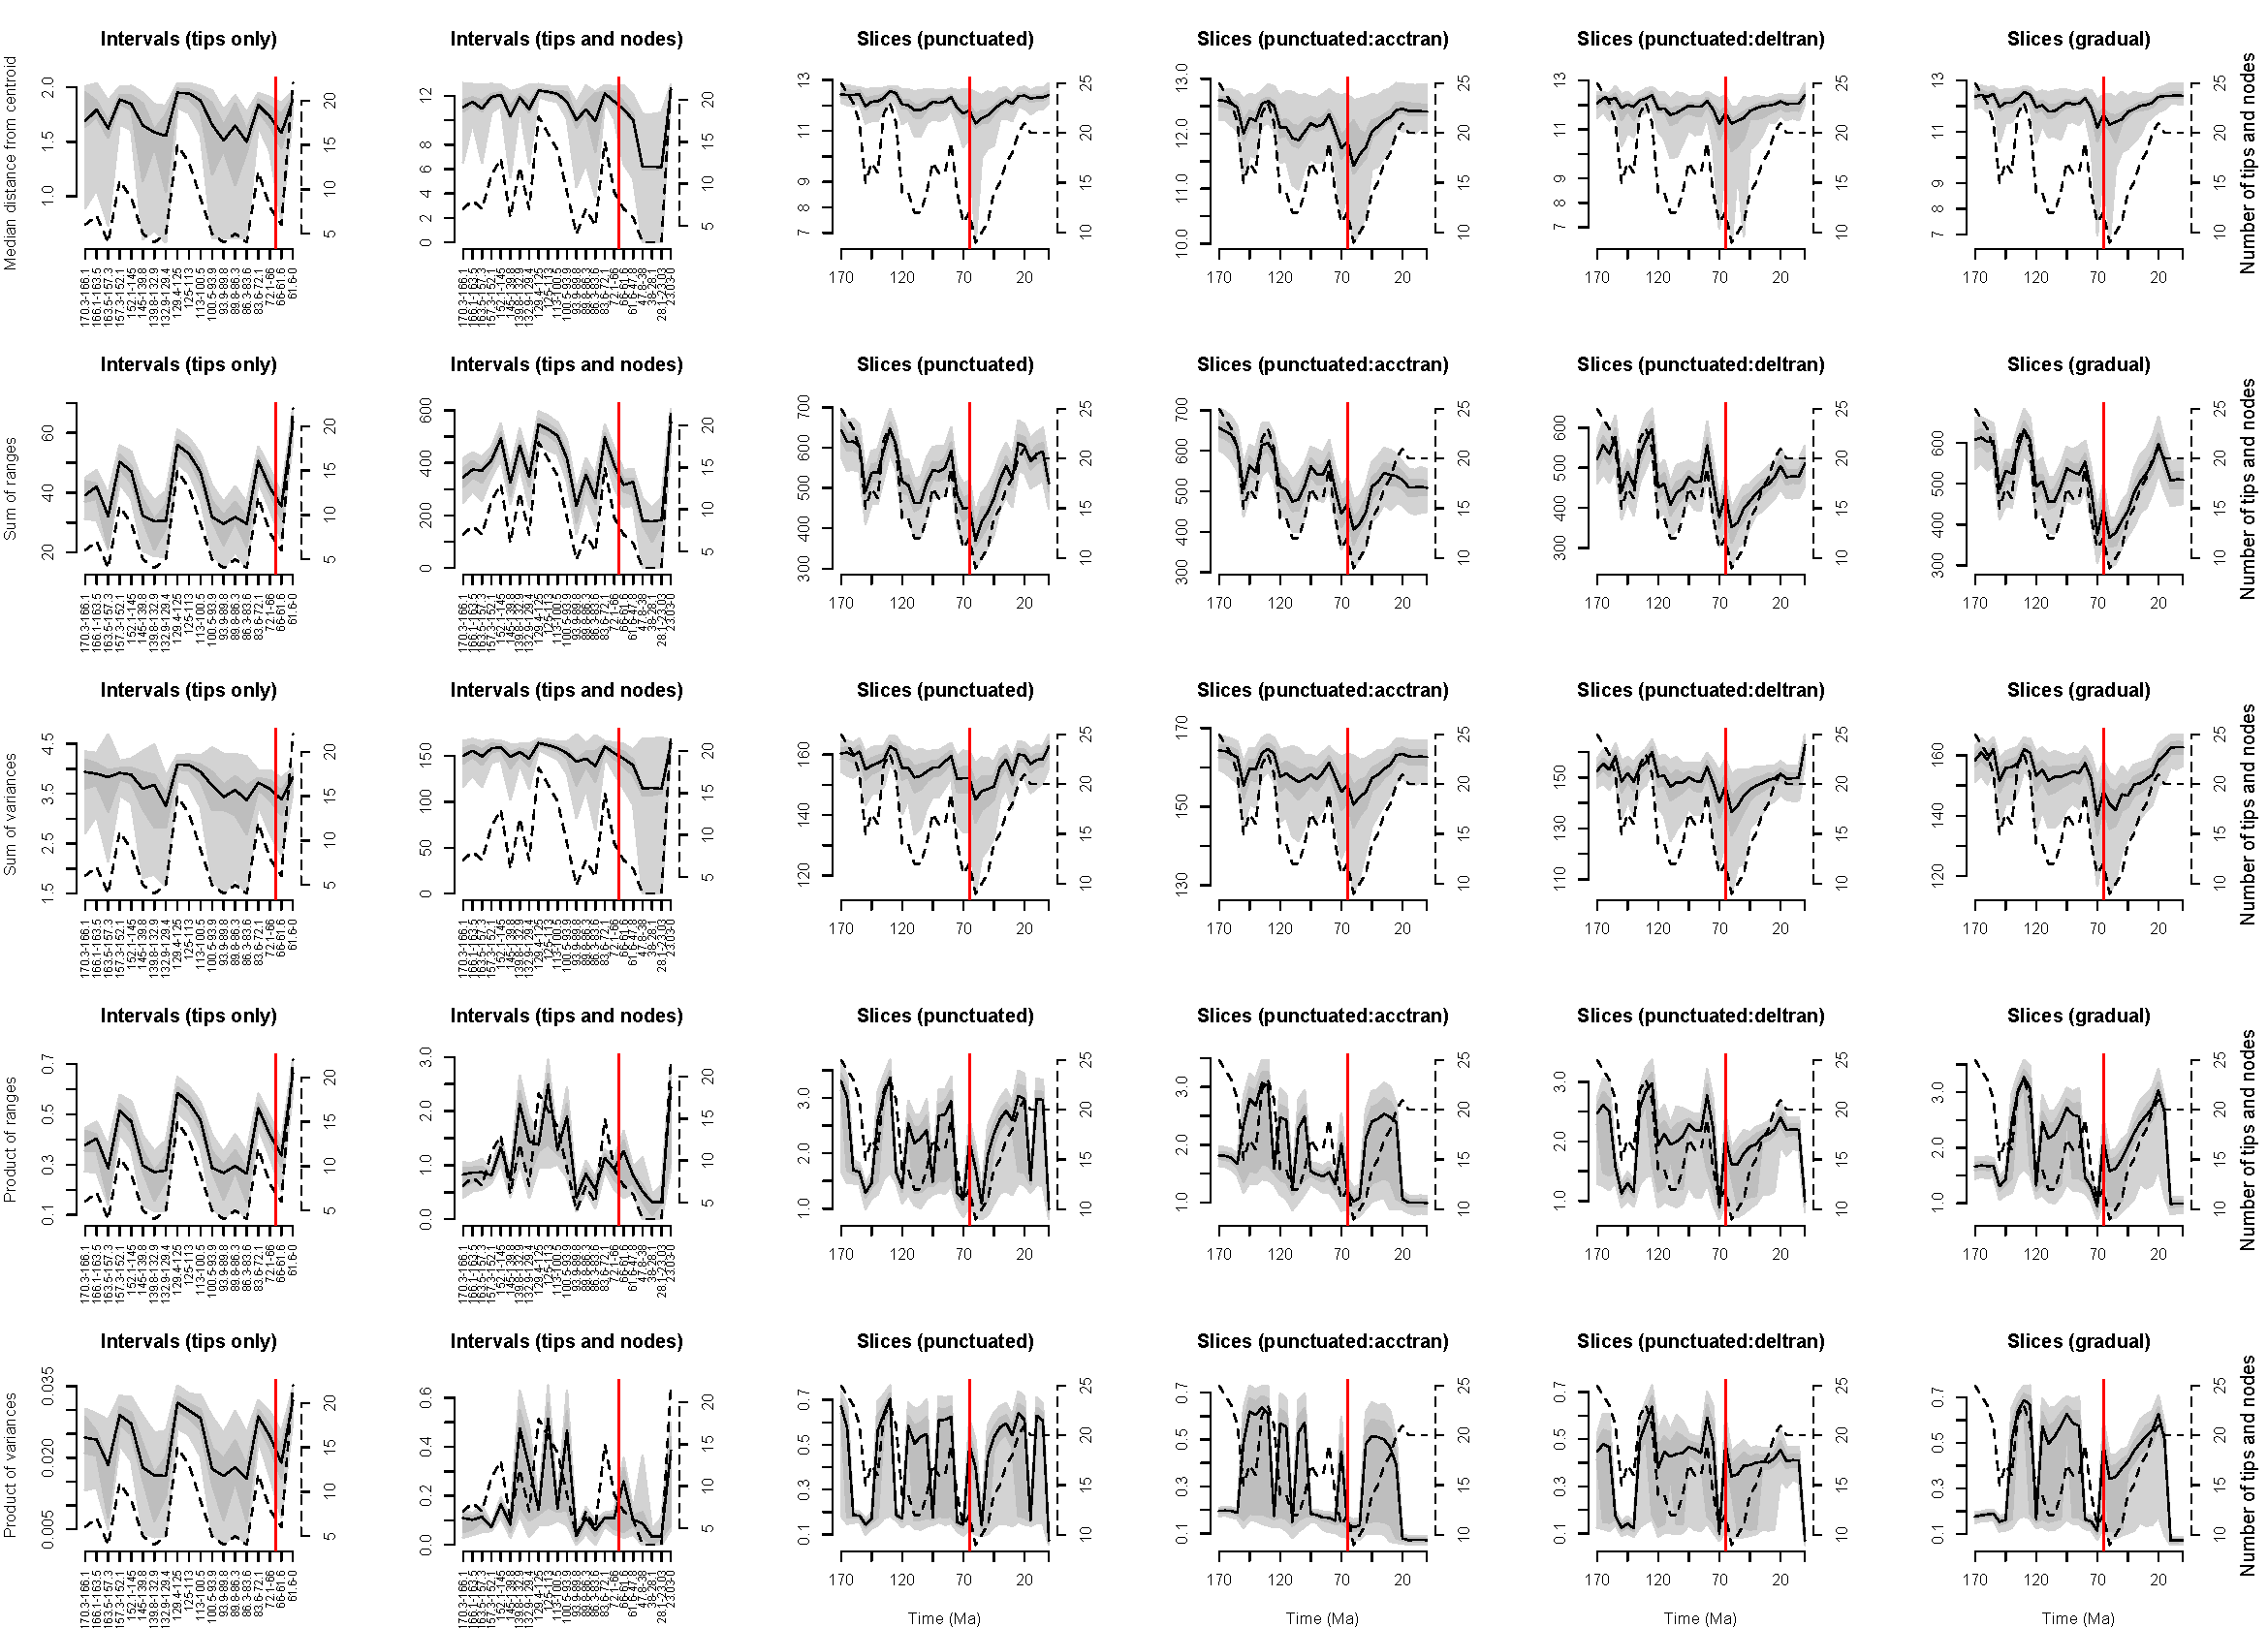
\includegraphics[width=\textwidth,height=\textheight,keepaspectratio]{Figures/Mammaliaformes(slater)_all_methods.pdf}
\caption{Variations of disparity through time among Mammaliaformes with disparity measurements and methods for sampling disparity through time. The x axis represents the time in Million of years ago (Mya). The y axis represents the disparity measured as the median distance from centroid per sub-sample. The solid black lines is the mean disparity; the confidence intervals (CI) are represent by the grey polygons (50\% CI in dark grey and 95\% CI in light grey). The dashed line represent the species richness in each sub-sample (values are reported on the right hand side of each graphs). The red vertical line represents the K-Pg boundary (66 Mya).}
\end{figure}
\end{landscape}

\begin{landscape}
\begin{figure}[!htbp]
\centering
    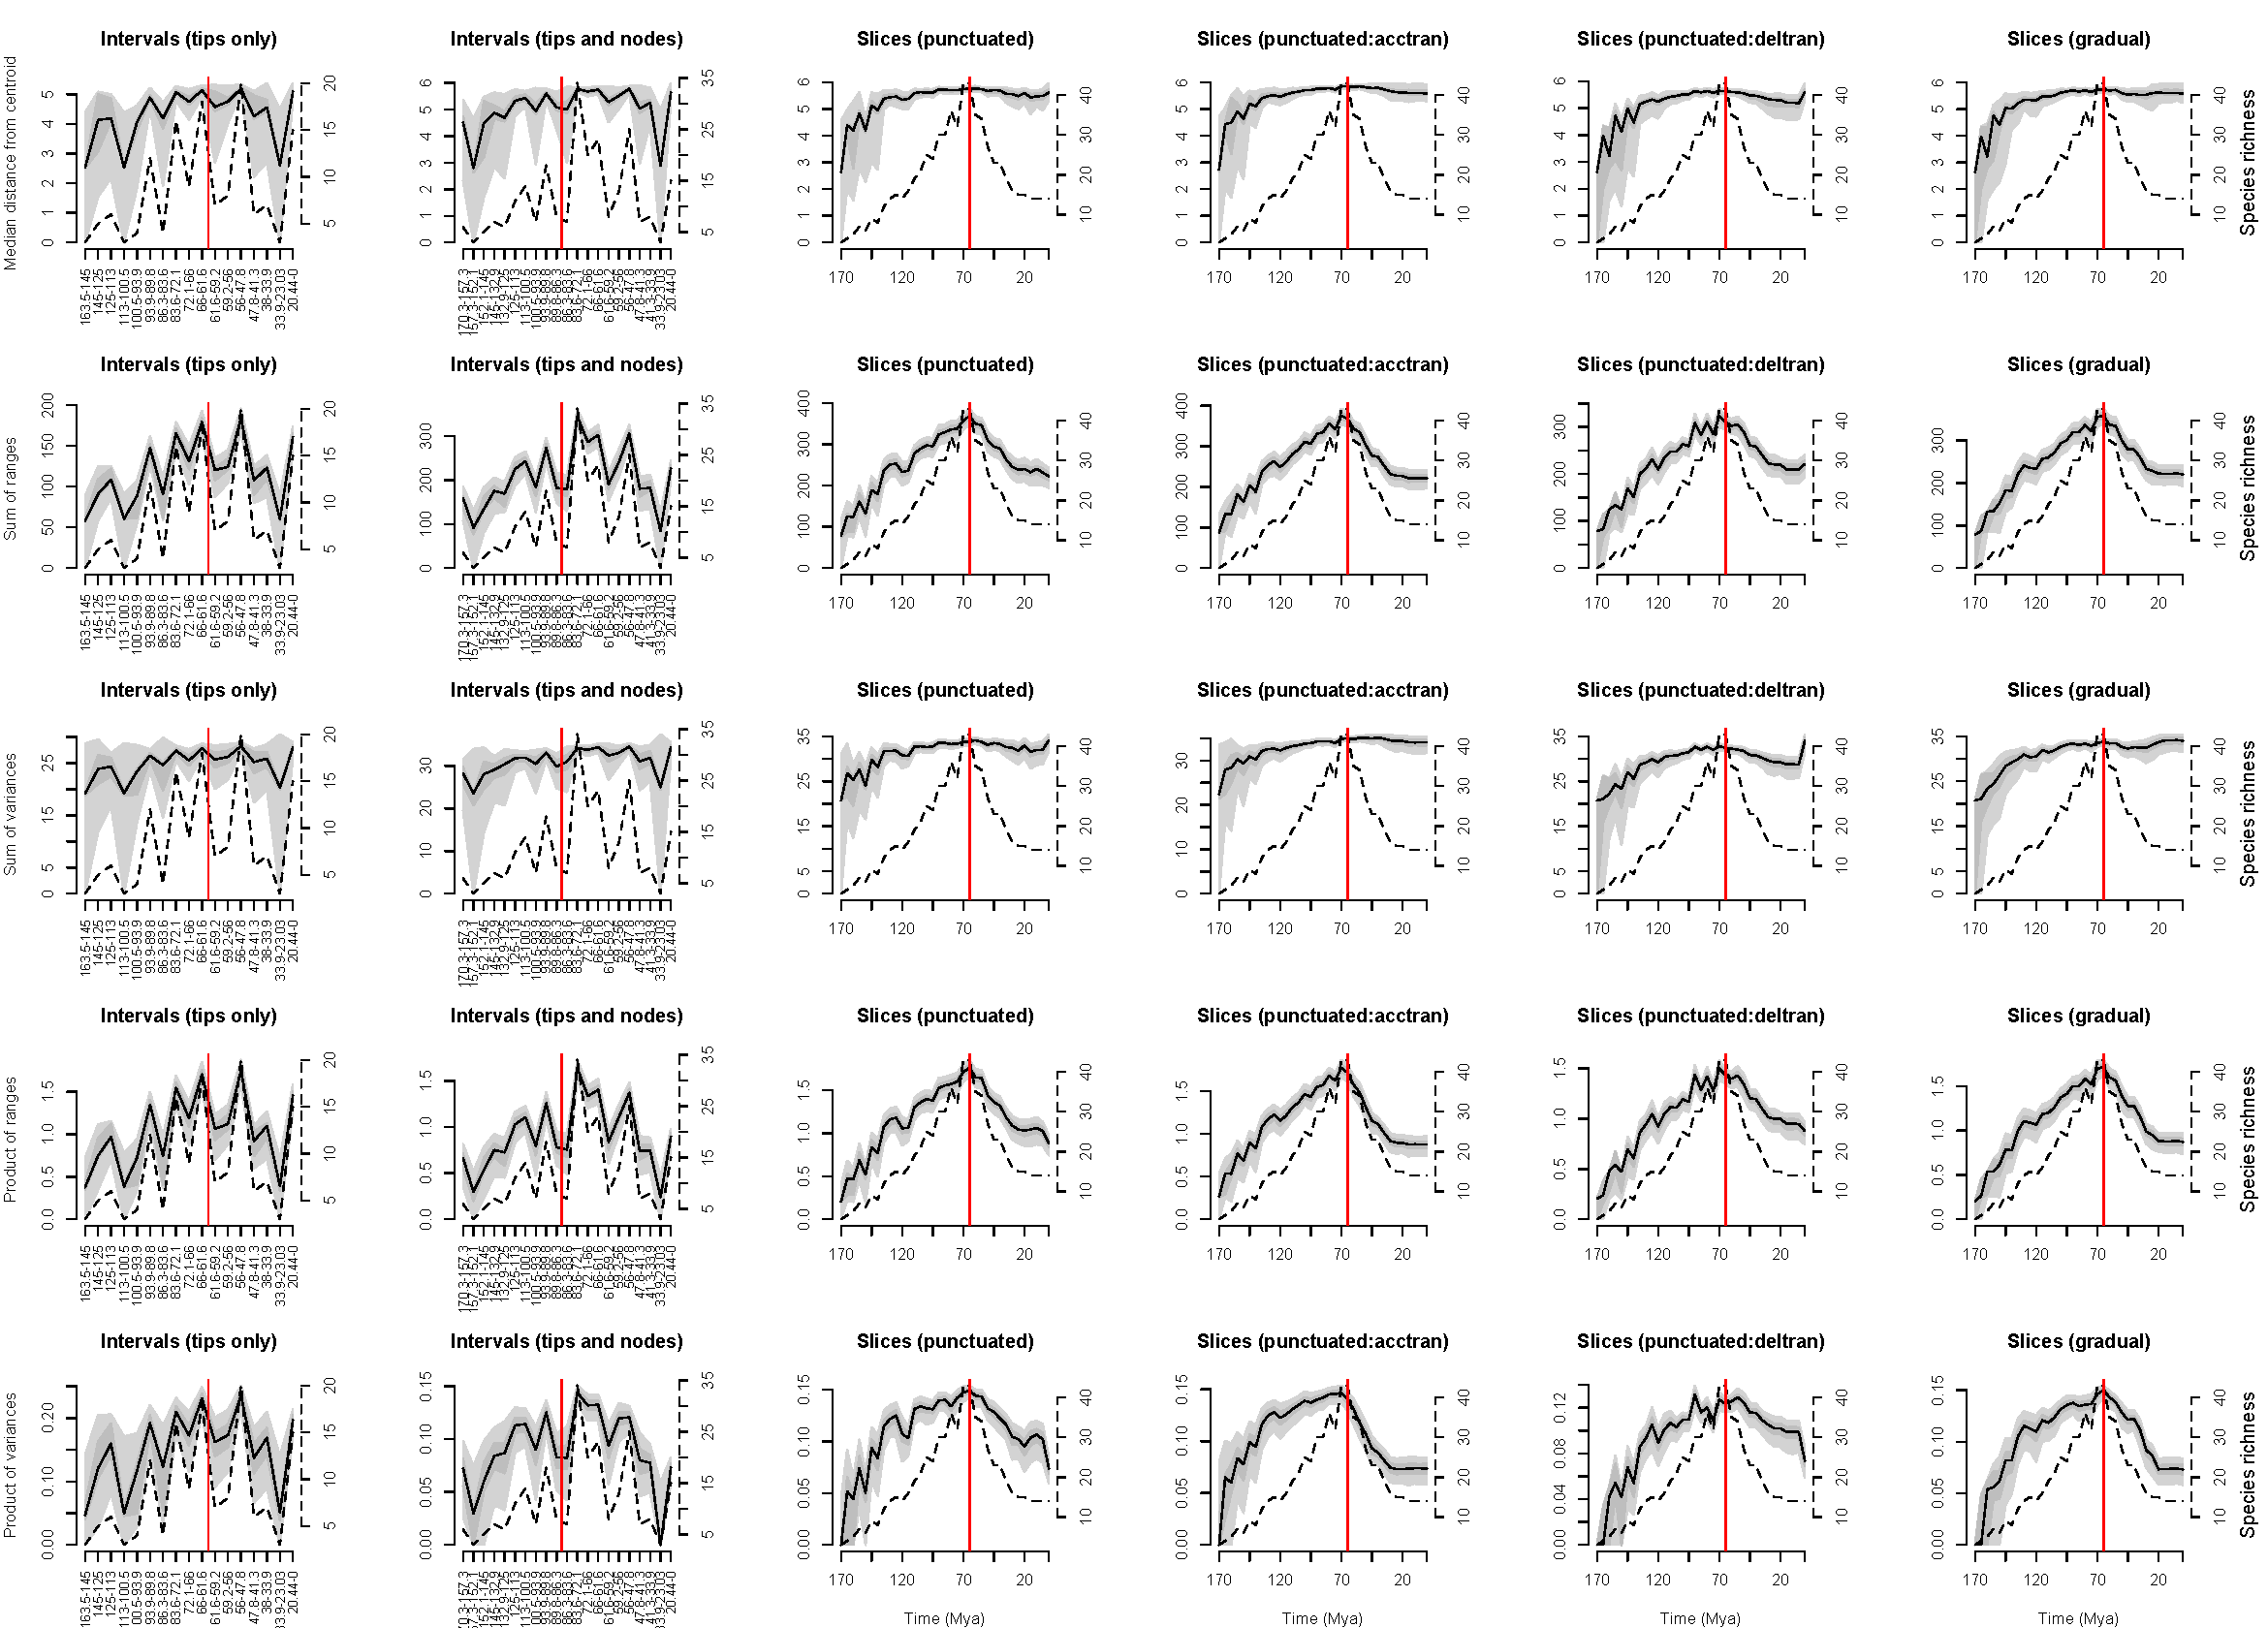
\includegraphics[width=\textwidth,height=\textheight,keepaspectratio]{Figures/Eutheria(beck)_all_methods.pdf}
\caption{Variations of disparity through time among Eutherian with disparity measurements and methods for sampling disparity through time. The x axis represents the time in Million of years ago (Mya). The y axis represents the disparity measured as the median distance from centroid per sub-sample. The solid black lines is the mean disparity; the confidence intervals (CI) are represent by the grey polygons (50\% CI in dark grey and 95\% CI in light grey). The dashed line represent the species richness in each sub-sample (values are reported on the right hand side of each graphs). The red vertical line represents the K-Pg boundary (66 Mya).}
\end{figure}
\end{landscape}

\begin{landscape}
\begin{figure}[!htbp]
\centering
    \includegraphics[width=\textwidth,height=\textheight,keepaspectratio]{Figures/Mammaliaformes(slater)_all_methods_rarefied.pdf}
\caption{Variations of disparity through time among Mammaliaformes with disparity measurements and methods for sampling disparity through time (rarefied with 3 taxa for the interval method and 8 taxa for the slice method). The x axis represents the time in Million of years ago (Mya). The y axis represents the disparity measured as the median distance from centroid per sub-sample. The solid black lines is the mean disparity; the confidence intervals (CI) are represent by the grey polygons (50\% CI in dark grey and 95\% CI in light grey). The dashed line represent the species richness in each sub-sample (values are reported on the right hand side of each graphs). The red vertical line represents the K-Pg boundary (66 Mya).}
\end{figure}
\end{landscape}

\begin{landscape}
\begin{figure}[!htbp]
\centering
    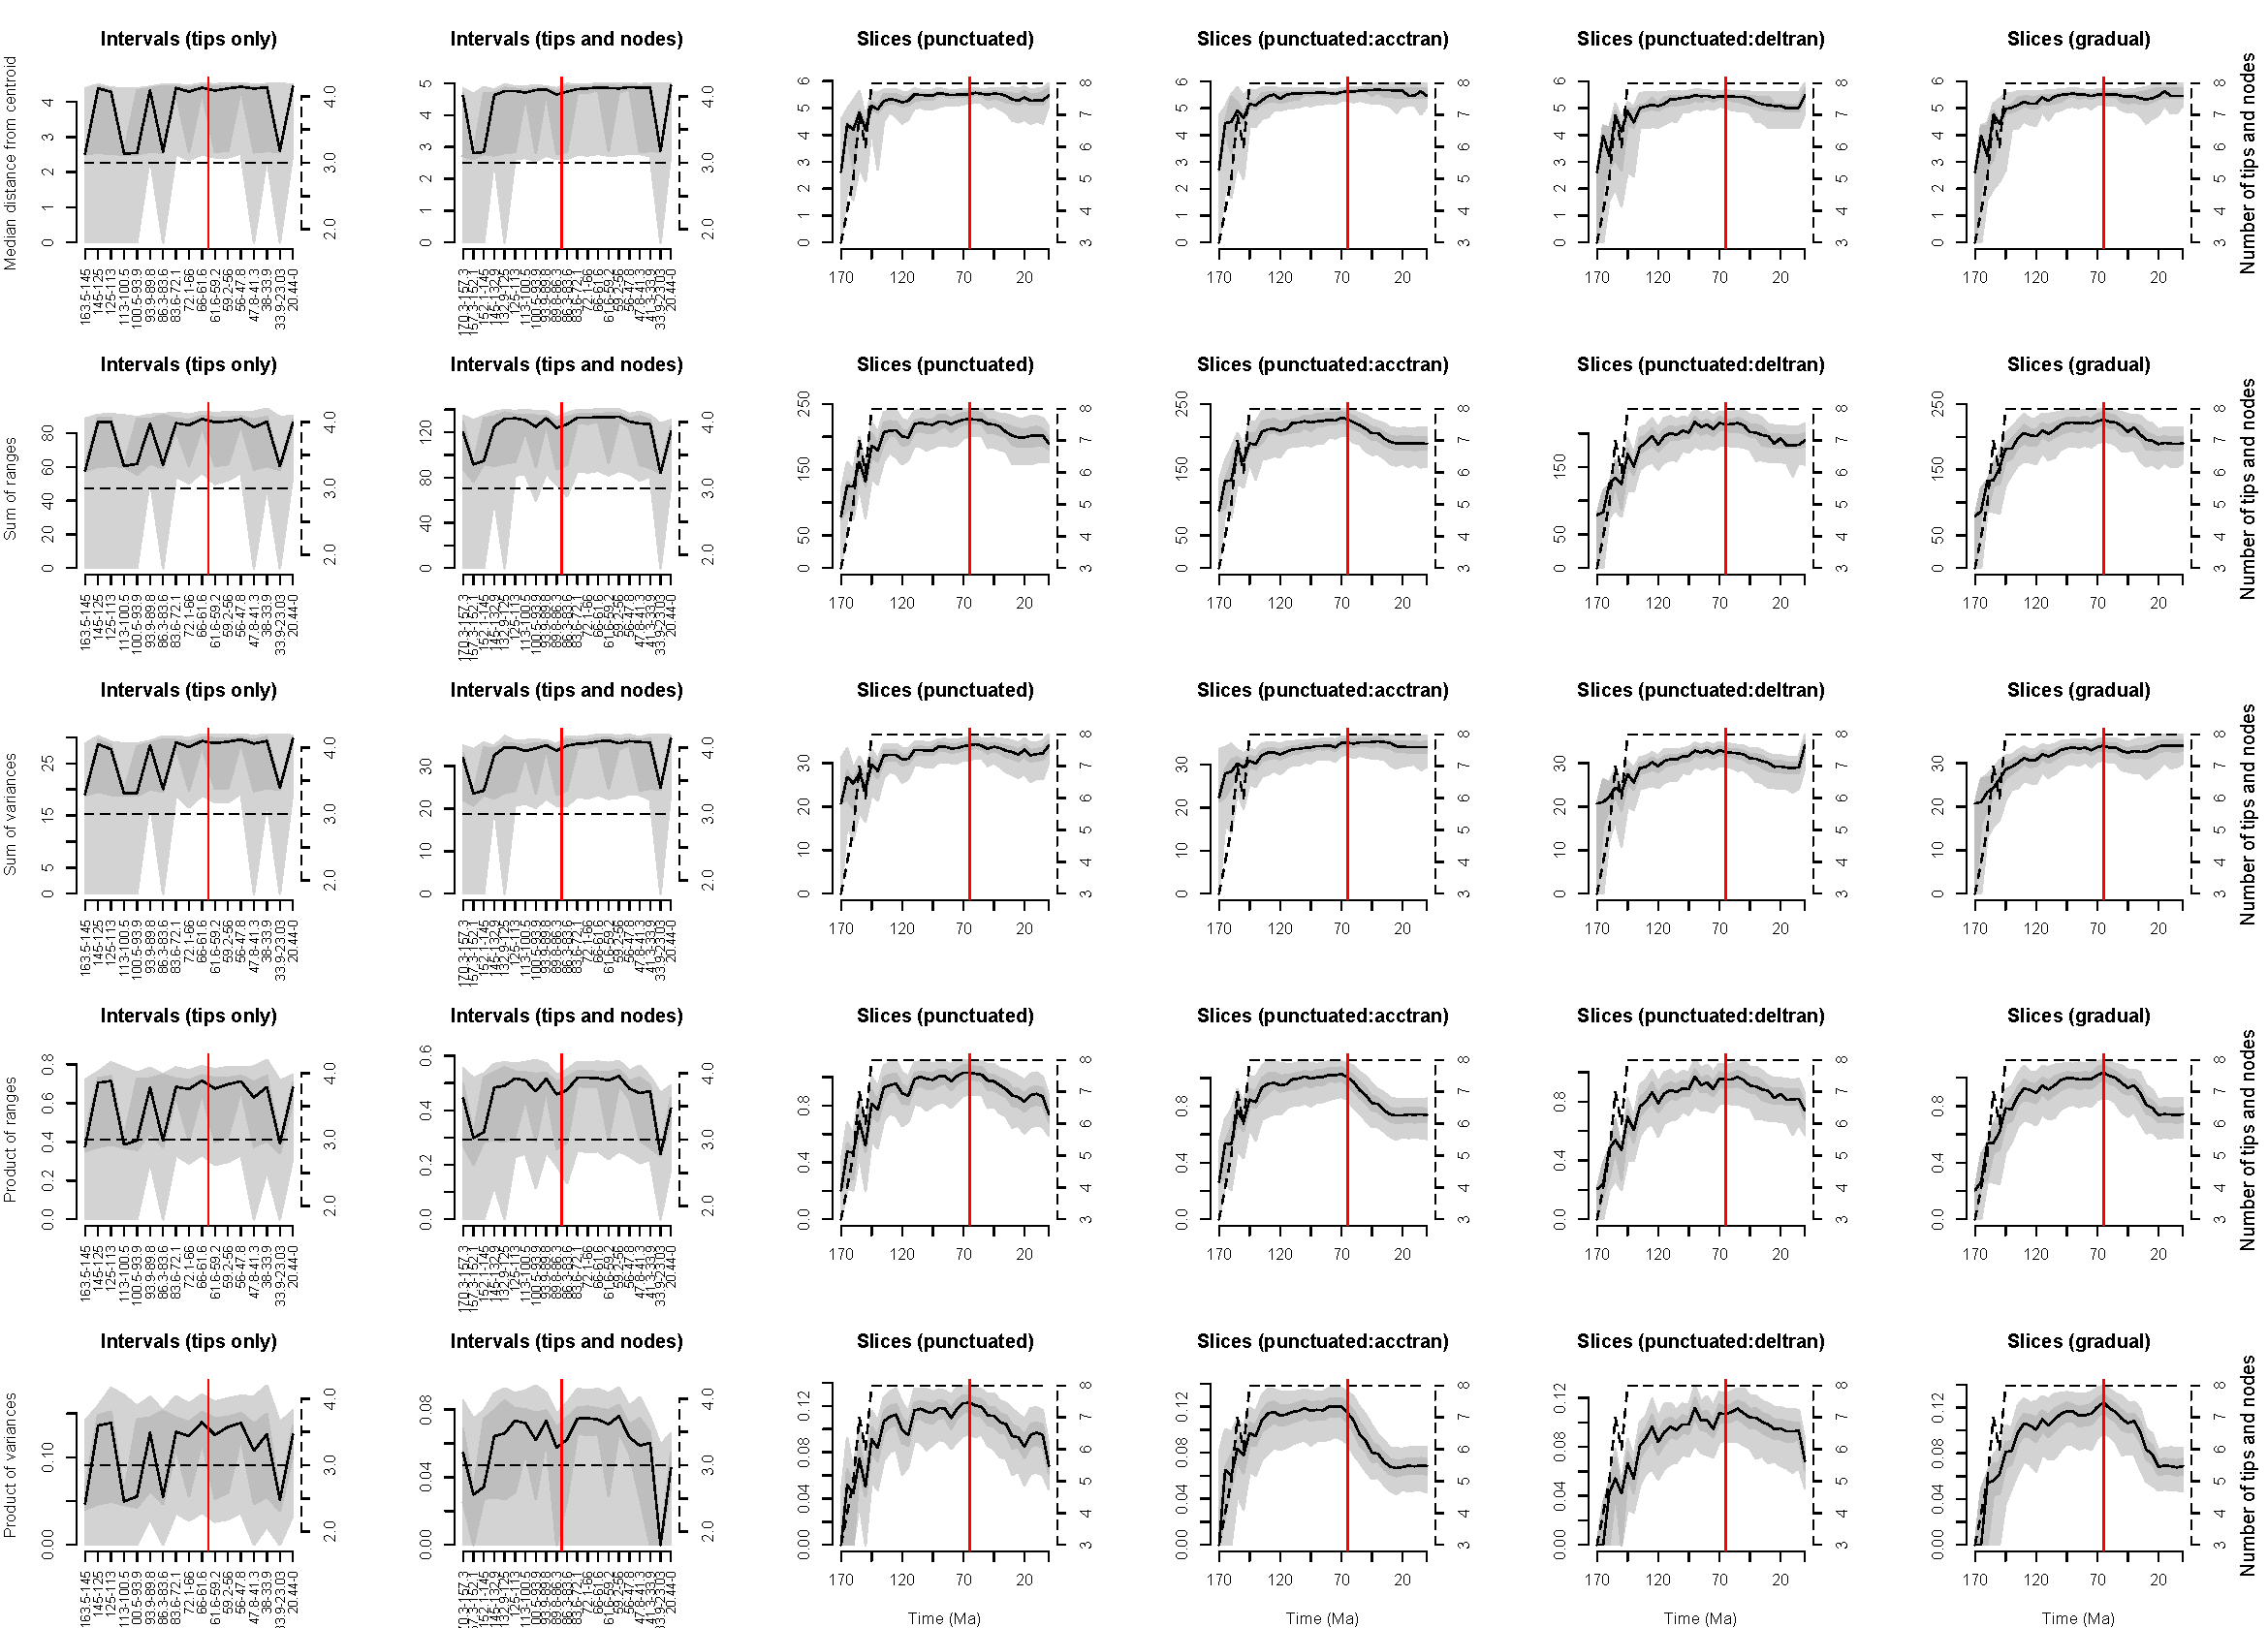
\includegraphics[width=\textwidth,height=\textheight,keepaspectratio]{Figures/Eutheria(beck)_all_methods_rarefied.pdf}
\caption{Variations of disparity through time among Eutherian with disparity measurements and methods for sampling disparity through time (rarefied with 3 taxa for the interval method and 8 taxa for the slice method). The x axis represents the time in Million of years ago (Mya). The y axis represents the disparity measured as the median distance from centroid per sub-sample. The solid black lines is the mean disparity; the confidence intervals (CI) are represent by the grey polygons (50\% CI in dark grey and 95\% CI in light grey). The dashed line represent the species richness in each sub-sample (values are reported on the right hand side of each graphs). The red vertical line represents the K-Pg boundary (66 Mya).}
\end{figure}
\end{landscape}


\bibliographystyle{sysbio}
\bibliography{References}


\end{document}